% !TEX root = ../ITGO.tex

%\subsection*{Tension/compression spring design problem}


This problem was introduced by \cite{TC}, and the objective is the minimization of the weight of a tension/compression spring (Figure \ref{fig:TC}). The problem has three continuous design variables, being them the diameter of spring wire ($x_1 = D$), the diameter of spring mean coil ($x_2 = d$) and the number of active coils ($x_3 = P$). It is subject to three nonlinear and one linear inequality constraints. The objective function value at the known global optimum is $f(\bm{x}^*) = 0.01266523$. The full mathematical formulation of the problem follows:

\vspace{-0.5cm}

\begin{align*}
\textbf{Minimize:} & \\
& f(\bm{x}) = (x_3 + 2)x_2x_1^2 \\[0.5em]
\textbf{subject to:} &\\
& g_1(\bm{x}) = 1 - \frac{x_2^3 x_3}{7.1785 x_1^4} \leq 0 \\
& g_2(\bm{x}) = \frac{4x_2^2 - x_1 x_2}{12,566 (x_2 x_1^3) - x_1^4} + \frac{1}{5.108 x_1^2} - 1 \leq 0 \\
& g_3(\bm{x}) = 1 - \frac{140.45 x_1}{x_2^2 x_3} \leq 0 \\
& g_4(\bm{x}) = \frac{x_2 + x_1}{1.5} - 1 \leq 0 \\[0.5em]
\textbf{with bounds:} & \\
& 0.05 \leq x_1 \leq 2, \quad 0.25 \leq x_2 \leq 1.3, \quad 2 \leq x_3 \leq 15
\end{align*}

\vspace{0.5cm}


\begin{figure}[h]
\begin{center}
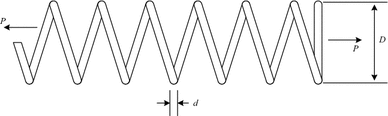
\includegraphics[scale=0.6]{img/Problems/TC.png}
\end{center}
\captionsetup{justification=centering}
\caption{Schematic view of the tension/compression spring design problem.}\label{fig:TC}
\end{figure}
